\chapter{Planning and Progress}

\section{Planning}

%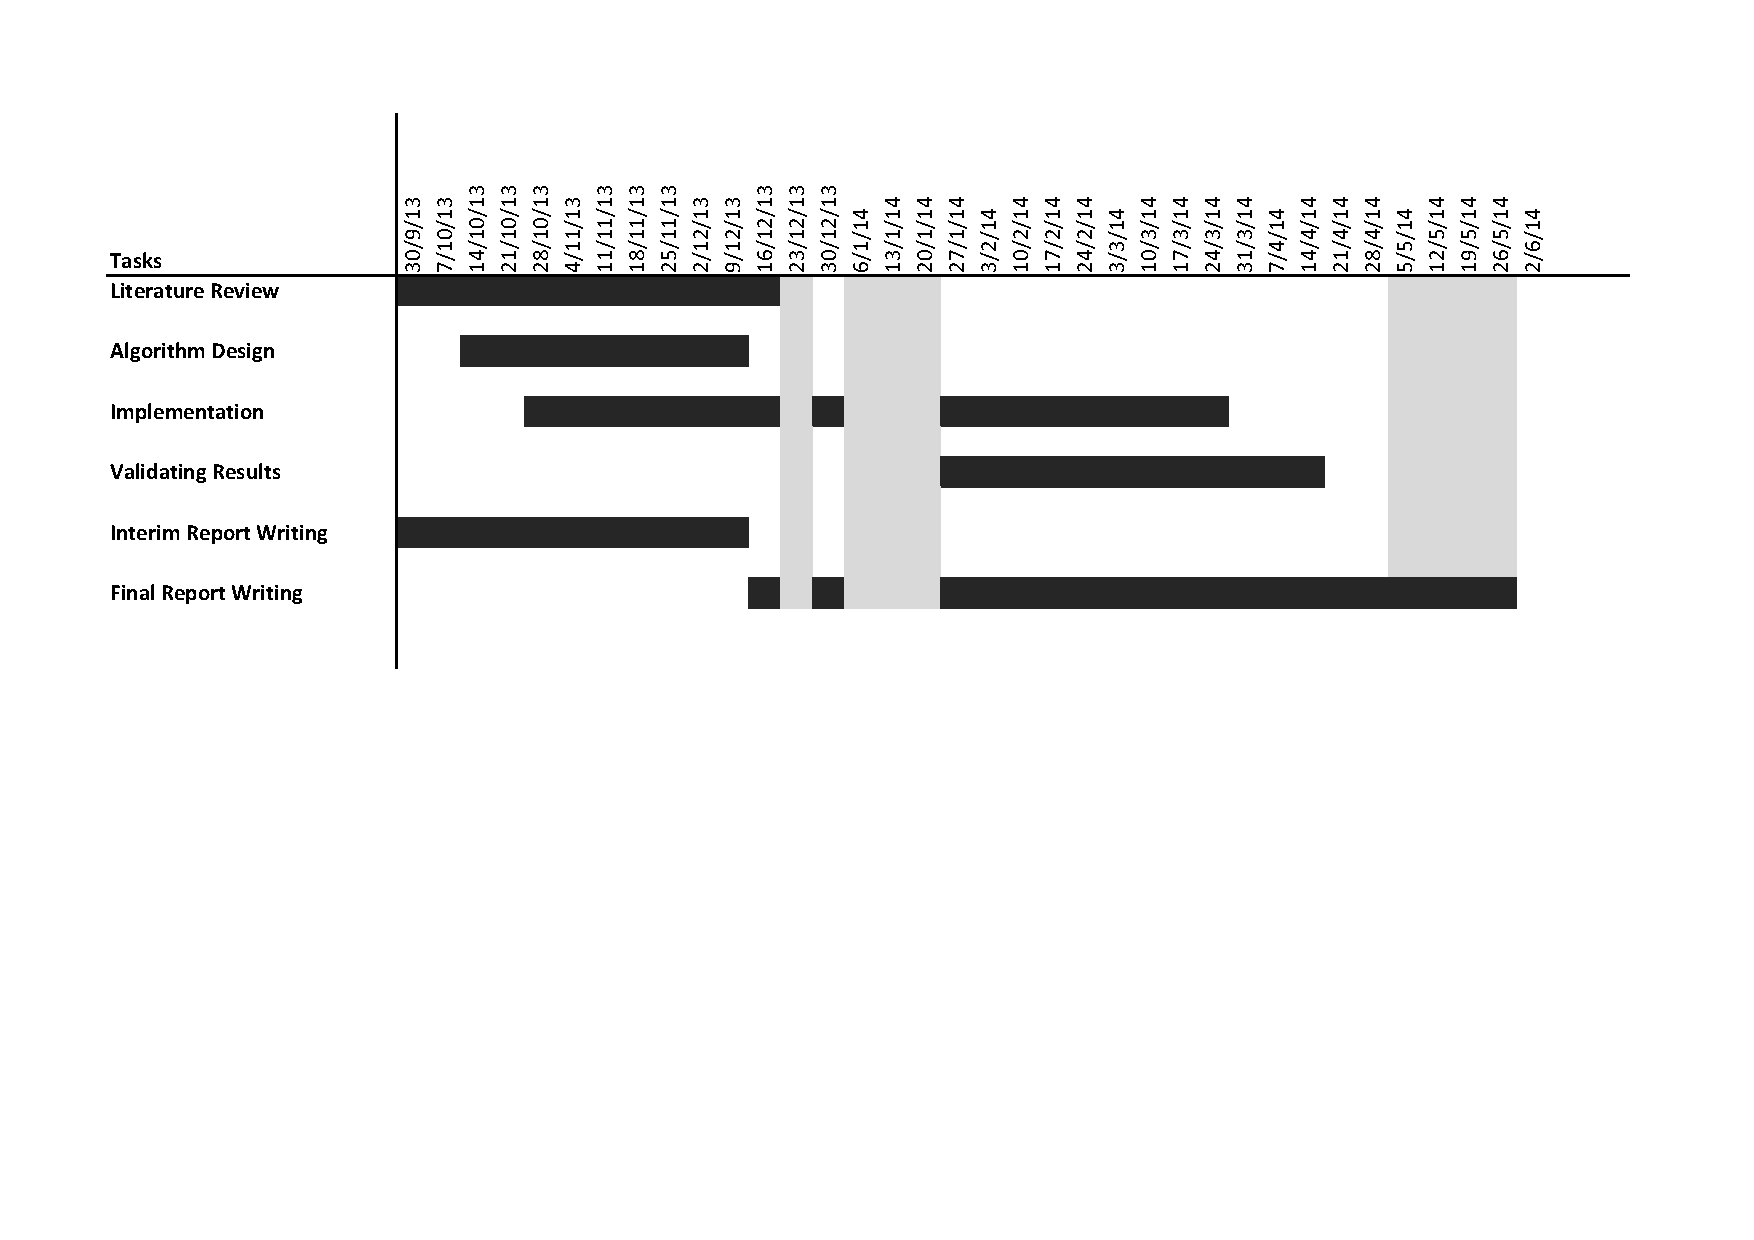
\includegraphics[width=1.1\linewidth]{images/planningGantt.pdf}

Figure \ref{planningGantt} is the original Gantt chart showing the general intended plan of progression through this project. A review of the current literature and other background research was to be done throughout the first term and most heavily concentrated at the beginning before the mathematical algorithm design should start. The algorithm was designed and implemented early on and ran in parallel with the implementation in software to allow for constant testing and verification of results. I planned to write the progress report over this whole period to spread out workload, but effort here would be focused at the end of the first term. The second term was dedicated to the continued software implementation and a testing and verification period. This allowed for time to develop the demonstration application and produce the final report over the Easter holiday. 

\begin{figure}[ht!]
    \makebox[\linewidth]{
       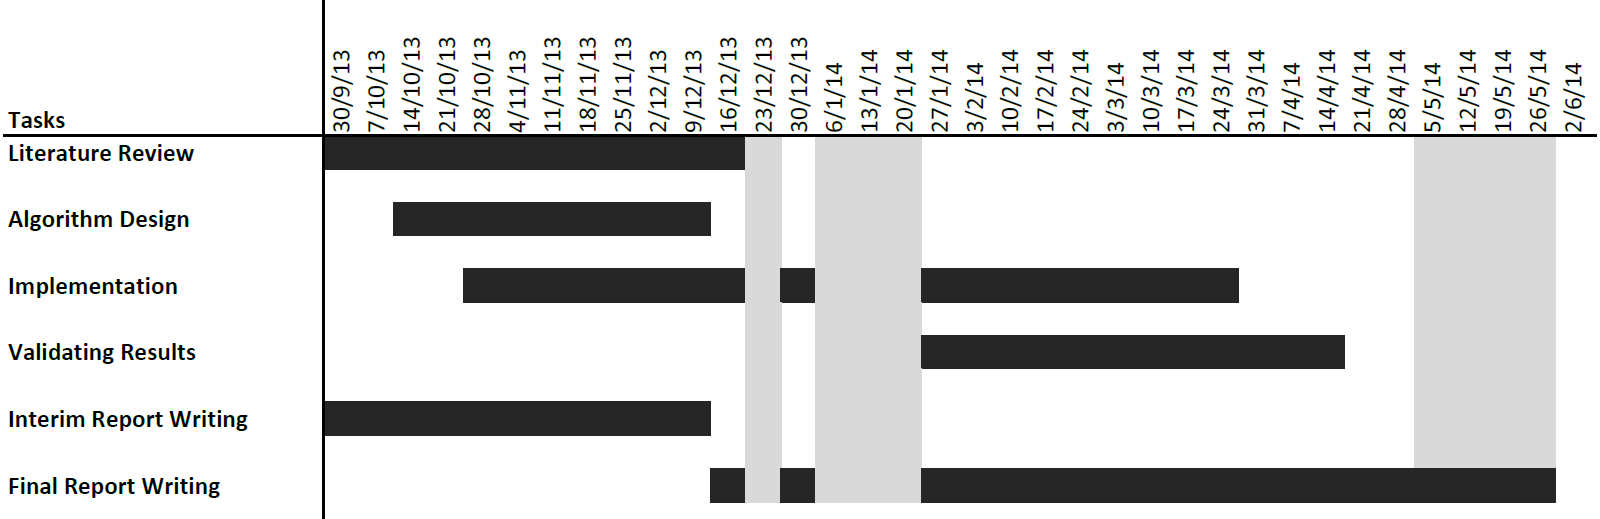
\includegraphics[width=1.0\linewidth]{images/planningGantt.png}
    }
    \caption{Gantt chart of planned work}
    \label{planningGantt}
\end{figure}

\section{Progress}

Preliminary work began with background research into recommender systems, content-based filtering and semantic analysis. Figure \ref{finalGantt} shows the breakdown of various aspects of the project in to their distinct constituent parts. Time was spent looking at existing content aggregators and some of the applications of recommender systems in order to establish a suitable direction for my research to take. Methods of scoring using both a collaborative approach and a content-based approach were considered. A period of investigation into text analysis techniques was undertaken, during which it became apparent that it would not be time efficient given the goals and time constraints of the project to manually design a text analysis library, but instead to use existing implementations. The acquisition of real-life data was considered in order to inform the design of the API and a suitable sorting algorithm was determined.

\begin{figure}[ht!]
    \makebox[\linewidth]{
       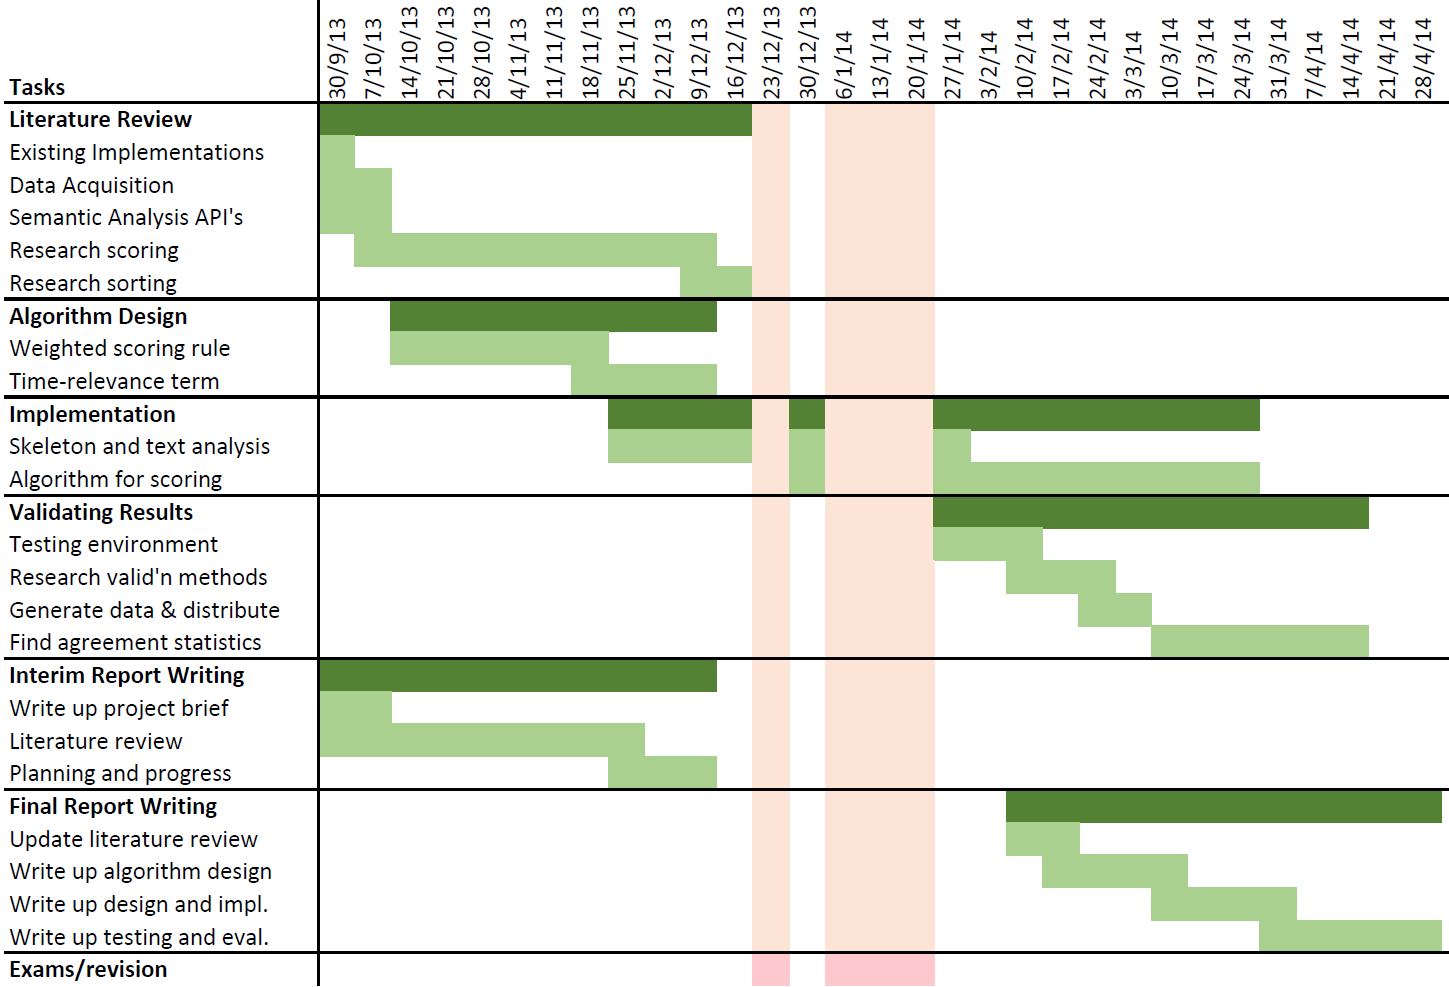
\includegraphics[width=1.0\linewidth]{images/finalGanttChart.png}
    }
    \caption{Gantt chart of planned work}
    \label{finalGantt}
\end{figure} 

Soon after, early versions of the recommender system were mathematically drafted out. Considerable time was devoted to choosing the broad approach that should be taken when considering a social media recommender system. This went on to involve the definition of important terms; the derivation using complex techniques the principles of weighted scoring; the justification of exponential time-related decaying terms and normalisation. All the while it was essential to consider the extent to which every approach would be able to be implemented on software. 

The next step was to implement the algorithm in software. Java was used as the language to implement the recommender system for its wide usage, ease of use and comprehensive capabilities. A JSON-based (JavaScript Object Notation) data manager was implemented next as the platform for test data, for its simple read- and write-ability. This required the redesign of part of the testing environment so as to load data by navigating an ordered file structure and loading data from these JSON files.

The testing of the behaviour of the recommender system was conducted in the last term before and during the Easter break. Kendall's $\tau$ (Eqn. \ref{KendallsTau}) was used as a quantitative measure of agreement in order to indicate the effectiveness of the algorithm. While additional extended amounts of testing could have been done to analyse some of the more special-case scenarios in which the algorithm could be used, testing has been completed to a good degree of comprehensiveness and is indicative of the anticipated predictive behaviour of the recommender system. Time was spent evaluating the test results and considering possible avenues of future work. 
